% Documentation of Infernal's Dirichlet prior file format
%
% Uses no sectioning commands, so it may be included as a subsection of
% a section, or a section in a chapter of file formats.
% The .tex file that includes this one provides the \section{} header.
%  
% SRE, Wed Apr  6 13:46:43 2005
% SVN $Id$

A prior file is parsed into a number of whitespace-delimited,
non-comment fields. These fields are then interpreted in order.  The
order and number of the fields is important. This is not a robust,
tag-value save file format.

All whitespace is ignored, including newlines. The number of fields
per line is unimportant.

Comments begin with a \verb+#+ character. The remainder of any line
following a \verb+#+ is ignored.

The Infernal source distribution includes an example prior file,
\prog{default.pri}. This prior is identical to the hardcoded default
prior used by Infernal. The following text may only make sense if
you're looking at that example while you read.

The order of the fields in the prior file is as follows:

\begin{description}
\item[\textbf{Strategy.}] The first field is the keyword
  \emprog{Dirichlet}. Currently Dirichlet priors (mixture or not)
  are the only prior strategy used by Infernal.

\item[\textbf{Transition prior section.}] The next field is the number
  \emprog{74}, the number of different types of transition
  distributions. (See Figure~\ref{fig:magic74} for an explanation of
  where the number 74 comes from.) Then, for each of these 74
  distributions:

  \begin{description}
  \item{\emprog{<from-uniqstate> <to-node>}:} Two fields give the
  transition type: from a unique state identifier, to a node
  identifier. Example: \emprog{MATP\_MP MATP}. 

  \item{\emprog{<n>}:} One field gives the number of transition
  probabilities for this transition type; that is, the number of
  Dirichlet parameter vector $\alpha^q_1..\alpha^q_n$ for each mixture
  component $q$.

  \item{\emprog{<nq>}:} One field gives the number of mixture
  Dirichlet components for this transition type's prior. Then,
  for each of these \emprog{nq} Dirichlet components:

     \begin{description}
     \item{\emprog{p(q)}:} One field gives the mixture coefficient $p(q)$,
     the prior probability of this component $q$. For a single-component
     ``mixture'', this is always 1.0.

     \item{$\mathbf{\alpha^q_1..\alpha^q_n}$:} The next $n$ fields give the
     Dirichlet parameter vector for this mixture component $q$.
     \end{description}
  \end{description}

\item[\textbf{Base pair emission prior section.}] This next section is
  the prior for MATP\_MP emissions. One field gives \emprog{<K>}, the
  ``alphabet size'' -- the number of base pair emission probabilities
  -- which is always 16 (4x4), for RNA. The next field gives \emprog{<nq>}, the
  number of mixture components. Then, for each of these \emprog{nq}
  Dirichlet components:
     \begin{description}
     \item{\emprog{p(q)}:} One field gives the mixture coefficient $p(q)$,
     the prior probability of this component $q$. For a single-component
     ``mixture'', this is always 1.0.

     \item{$\mathbf{\alpha^q_{AA}..\alpha^q_{UU}}$:} The next 16 fields give the
     Dirichlet parameter vector for this mixture component, in alphabetical
     order (AA, AC, AG, AU, CA \ldots GU, UA, UC, UG, UU). 
     \end{description}

\item[\textbf{Consensus singlet base emission prior section.}] This
  next section is the prior for MATL\_ML and MATR\_MR emissions.  One
  field gives \emprog{<K>}, the ``alphabet size'' -- the number of
  singlet emission probabilities -- which is always 4, for RNA.  The
  next field gives \emprog{<nq>}, the number of mixture components. Then,
  for each of these \emprog{nq} Dirichlet components:
     \begin{description}
     \item{\emprog{p(q)}:} One field gives the mixture coefficient $p(q)$,
     the prior probability of this component $q$. For a single-component
     ``mixture'', this is always 1.0.

     \item{$\mathbf{\alpha^q_A..\alpha^q_U}$:} The next 4 fields give the
     Dirichlet parameter vector for this mixture component, in alphabetical
     order (A, C, G, U).
     \end{description}
  
\item[\textbf{Nonconsensus singlet base emission prior section.}] This
  next section is the prior for insertions (MATP\_IL, MATP\_IR,
  MATL\_IL, MATR\_IR, ROOT\_IL, ROOT\_IR, BEGR\_IL) as well as
  nonconsensus singlets (MATP\_ML, MATP\_MR). 
  One field gives \emprog{<K>}, the ``alphabet size'' -- the number of
  singlet emission probabilities -- which is always 4, for RNA. 
  The next field gives \emprog{<nq>}, the
  number of mixture components. Then, for each of these \emprog{nq}
  Dirichlet components:
     \begin{description}
     \item{\emprog{p(q)}:} One field gives the mixture coefficient $p(q)$,
     the prior probability of this component $q$. For a single-component
     ``mixture'', this is always 1.0.

     \item{$\mathbf{\alpha^q_A..\alpha^q_U}$:} The next 4 fields give the
     Dirichlet parameter vector for this mixture component, in alphabetical
     order (A, C, G, U).
     \end{description}
\end{description}


\begin{figure}[htp]
\begin{center}
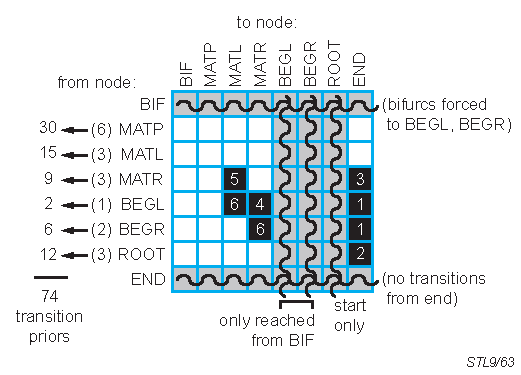
\includegraphics{Figures/stl9-63}
\end{center}
\caption{\small\textbf{Where does the magic number of 74 transition
distribution types come from?} The transition distributions are
indexed in a 2D array, from a unique statetype (20 possible) to a
downstream node (8 possible), so the total conceivable number of
different distributions is $20 \times 8 = 160$. The grid represents
these possibilities by showing the $8 \times 8$ array of all node
types to all node types; each starting node contains 1 or more unique
states (number in parentheses to the left).
Two rows are impossible (gray): bifurcations automatically transit to
determined BEGL, BEGR states with probability 1, and end nodes have no
transitions.  Three columns are impossible (gray): BEGL and BEGR can
only be reached by probability 1 transitions from a bifurcation, and
the ROOT node is special and can only start a model. 
Eight individual cells of the grid are unused (black) because of the
way \prog{cmbuild} (almost) unambiguously constructs a guide tree from
a consensus structure.  These cases are numbered as follows. (1) BEGL
and BEGR never transit to END; this would imply an empty
substructure. A bifurcation is only used if both sides of the split
contain at least one consensus pair (MATP). (2) ROOT never transits to
END; this would imply an alignment with zero consensus
columns. Infernal models assume $\geq 1$ consensus columns. (3) MATR
never transits to END. Infernal always uses MATL for unpaired columns
whenever possible. MATR is only used for internal loops,
multifurcation loops, and 3' bulges, so MATR must always be followed
by a BIF, MATP, or another MATR. (4) BEGL never transits to MATR. The
single stranded region between two bifurcated stems is unambiguously
assigned to MATL nodes on the right side of the split, not to MATR
nodes on the left. (5) MATR never transits to MATL. The only place
where this could arise (given that we already specified that MATL is
used whenever possible) is in an interior loop; there, by unambiguous
convention, MATL nodes precede MATR nodes. (6) BEGL nodes never
transit to MATL, and BEGR nodes never transit to MATR. By convention,
at any bifurcated subsequence $i,j$, $i$ and $j$ are paired but not to
each other. That is, the smallest possible subsequence is bifurcated,
so that any single stranded stretches to the left and right are
assigned to MATL and MATR nodes above the bifurcation, instead of MATL
nodes below the BEGL and MATR nodes below the BEGR.
Thus, the total number 74 comes from multiplying, for each row, the
number of unique states in each starting node by the number of
possible downstream nodes (white), and summing these up, as shown to
the left of the grid.}
\label{fig:magic74}
\end{figure}